\documentclass[a4paper,11pt]{article}

% \usepackage[lf]{Baskervaldx}       % text
% \usepackage[bigdelims,vvarbb]{newtxmath} % math
% \usepackage[cal=boondoxo]{mathalfa}      % \mathcal

\usepackage[T1]{fontenc}
\usepackage{baskervillef}                 % text
\usepackage[baskerville,vvarbb]{newtxmath} % math tuned for BaskervilleF
\usepackage[cal=boondoxo]{mathalfa}

\usepackage{microtype}
\usepackage{graphicx}
\graphicspath{{FIG/}}
\usepackage{amsmath} % don't load amssymb with unicode-math

\usepackage{color}
\usepackage[table]{xcolor}
\usepackage{eso-pic}
\usepackage{longtable}
\usepackage{sidecap}

\setlength{\fboxsep}{3pt}
\tolerance=1000000
\hyphenpenalty=5000
\setcounter{tocdepth}{2}

\definecolor{lightblue}{rgb}{.94,.94,1.}
\definecolor{lightgreen}{rgb}{1.,.94,.94}
\definecolor{green}{rgb}{.94,1.,.94}
\definecolor{bluemy2}{rgb}{0.,0.,0.4}
\definecolor{redmy2}{rgb}{0.7,0.1,0.}
\definecolor{gray1}{rgb}{0.4,0.4,0.4}
\definecolor{graybox}{rgb}{0.94,0.94,0.94}
\definecolor{refcolor}{rgb}{0.3,0.3,0.3}

\usepackage{hyperref}
\hypersetup{
  pdftitle={Human-led Science in the Age of Superintelligence},
  pdfauthor={Vladislav A. Yastrebov},
  pdfsubject={Superintelligence, Science},
  pdfcreator={LaTeX},
  pdfkeywords={Superintelligence, Science, Human Science, Purpose and meaning, Frontiers of knowledge},
  pdfnewwindow=true,
  colorlinks=true,
  linkcolor=refcolor,
  citecolor=refcolor,
  filecolor=refcolor,
  urlcolor=refcolor
}
\usepackage{cleveref}

\let\openbox\relax

\usepackage{amsthm}
\newtheorem{hypothesis}{Hypothesis}

% Optional: nicer refs
\usepackage{cleveref}
\crefname{hypothesis}{Hypothesis}{Hypotheses}



\newcommand{\ie}{\emph{i.e.\ }}
\newcommand{\eg}{\emph{e.g.\ }}
\newcommand{\etc}{\emph{etc.\ }}
\newcommand{\etal}{\emph{et al.\ }}

\usepackage{nomencl}
\makenomenclature

\usepackage[backend=biber,style=authoryear,dashed=false]{biblatex}
\addbibresource{references.bib}
\DeclareDelimFormat{nameyeardelim}{\addcomma\space}

\title{Human's Science in the Age of Superintelligence}
\author{Vladislav A. Yastrebov}
\date{Sant Cugat del Vall\`es, Spain, August 2025}

\begin{document}

\maketitle
\begin{center}
    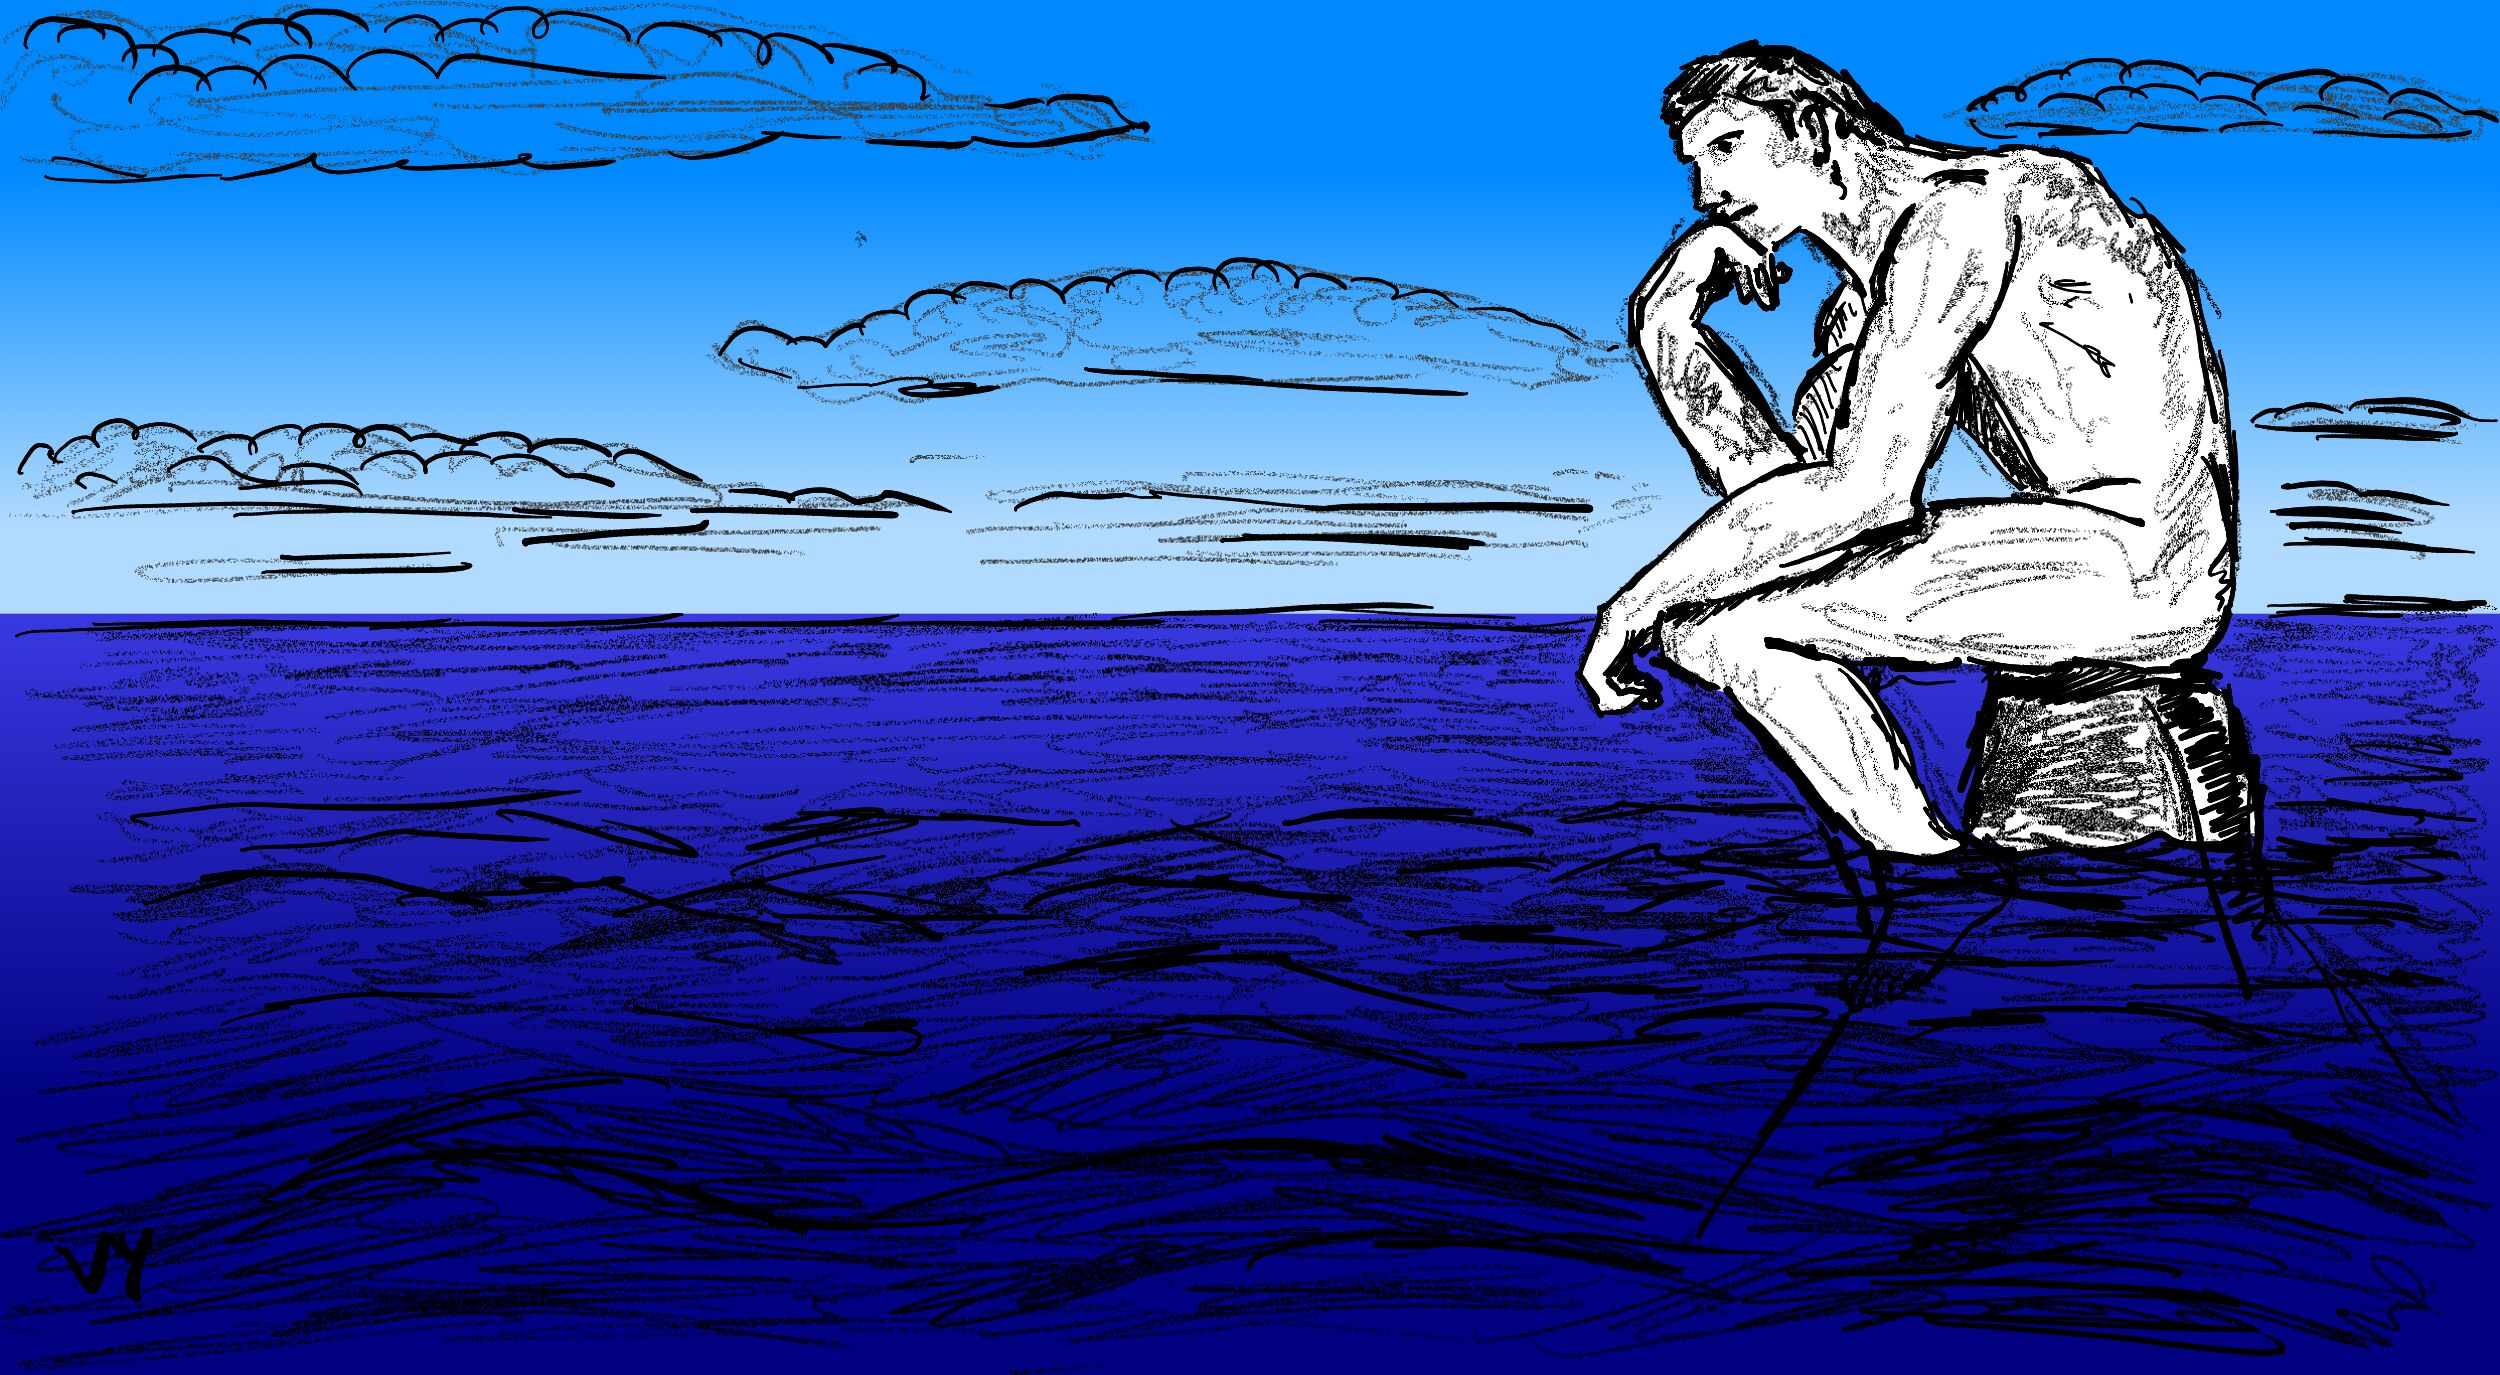
\includegraphics[width=1\textwidth]{Fig_SI_2.jpg}
    \footnotesize A Thinker on the Mount Everest's Summit\footnote{This figure refers to an analogy of a flooded landscape of human cognitive capacities, when the level of water is above a mountain of some capacities made better by machines than humans it is shown as flooded, the waxing crescent moon signifies a dawn of the human intellectual domination (well this interpretation of the crescent moon makes sense in the Northern hemisphere, and thus on the altitude of Mount Everest). [Ref, see Tegmark] }
\end{center}
    \newpage
 	\tableofcontents


    \printnomenclature

    \section{Raw}

    Current technology is already great and can get us rapidly much further in scientific progress. The technology develops too fast to let most of scientists catch up with its development pace.

    In many scenarios, in the world of SI \nomenclature{SI}{Superintelligence}, most of human activities transform into a game, the same gamification is expected for the science, one of the most serious and demanding humans occupations.
    
    It will be an utopian essay\footnote{Probably, for people not familiar with the concept of post-instrumental deep utopia from Bostrom, this text will see too far beyond their short-term imagination. So, I would invite them to take a look on the concepts and tools introduced in \textcite{DeepUtopia}.} in the spirit of~\parencite{DeepUtopia} and \parencite{LovingGrace}, but we shall not forget that getting to this utopian state with a friendly SI presents \textit{per se} a great challenge -- the most important and the last challenge that the humanity will face. However, the objective of this essay is to reflect on the state of science when this "great filter" has been overcame and the humanity has a well-aligned SI at its disposal \parencite{Yudkowsky2008,Yampolskiy2016,Yudkowsky2022}. Let's dream.

    Oracle type SI -- human scientists will ask intelligent question, accumulate knowledge, synthetize it and make progress in Science, but it seems that the AI\nomenclature{AI}{Artificial Intelligence in a general sense} development has not selected this path of development and a path of superpowerful and agentic "souverain" type, introduced by \textcite{Bostrom2014}, will prevail.

    With an SI, it is clear that the mankind is practically excluded from the advancement of the forefront science in important domains -- those which a critical for constructing an accurate world model. Then, will such occupation as "scientist" disappear completely? Probably not, because in a "solved world" a search for meaning will be crucial thought largely simplified by the SI, and a science-related occupation seems very appealing for those who value intelligence.

    Why SI will take lead in the scientific research? As known from~\parencite{Bostrom2014,Tegmark2017}, any goal provided to an AI -- super optimizer -- induces sub-goals such as self-preservation, access to resources and construction of an accurate world model.
    Nevertheless, it does not mean that all questions that are interesting for us, are not for this world model. Therefore, some scientific progress of the SI can ignore some questions asked by humans. Nevertheless, the SI could be managed to make progress in this directions if needed. Such class of scientific domains and questions we will denote as  idle scientific questions/domains.

    [Can I cite something from Grinbaum?]

\textbf{Fractal granularity of scientific landscape and its boundary}


    The pavement of scientific knowledge, or more specifically the boundary between known and unknown, between the ``terra cognita'' and ``terra incognita'', can be seen to some extent as a fractal surface in the sense that at the macroscopic scale of global domains we have a general understanding, on the smaller scale of particular details, we have a more detailed understanding and on smaller, microscopic scales we can have very specific questions, which for example can yet remain unanswered. Formulation and solution of such questions can lead to the refinement of our understanding, development of new methods and experiments, and even lead to new important subquestions\footnote{``The purpose of
models is not to fit the data but to sharpen the questions'', Samuel Karlin} representing further scales in this fractal knowledge landscape and eventually to some relevant discoveries. These small scales are critical for the advancement of the science. This fractal boundary between the known and unknown is fuzzy on the bigger scale and becomes clear on the smaller scales of specific questions. So, the advancement of the boundary can be ensured by clarifying these smaller scales. And an SI can see clearly the voids on these smaller scales and fill them in thus resulting to the gradual progress of the forefront. For the gradual and steady progress of the science, the amplitude of oscillations (standard deviation of the small scales from the average boundary) between the known and unknown shall be small enough. So I guess the frontiers of the SI-led science (SIS) can be smoother than this of the human-led Science (HS).

\textbf{Separation of HS and SIS}

It is essential to separate the SI-led Science (SIS) and the Human-led Science (HS). In the current HS, of course, nobody has a fine-granular understanding of the fractal boundary between the known and unknown but some scientists have a relatively broad vision of the fuzzy macroscale frontier at least in their own and neighbouring domains. Some scientists really work on the forefront of the global HS frontier, and some are simply pushing their own boundaries which are located in the vicinity of already known. If asked, SI will be able to bring scientists to the forefront or at least closer to the forefront of HS or SIS. Currently, the HS' frontier can be cristallized but of course it exists nowhere but in the global and cleanedup scientific literature. Therefore, individual scientific boundary and the global HS' even at the smaller scales can differ drastically. Now, we need to imagine that the SIS' boundary spanning all domains, at least those relevant to the world model construction, will further differ from the HS' boundary. Can the humanity assume that this new frontier belongs to them too? Probably not, since there's none of living or had lived human individuals who understood (in a broad sense of this verb) this new boundary or made progress from the HS' frontier to the SIS' one. Therefore, one of possible human's occupation will be pushing the HS' frontiers closer to the SIS' one.

Sharing of information between HS and SIS is not symmetric. If eventually, by chance, humans make progress beyond the SIS' frontier, the later can readily integrate this progress. The opposite is not possible, the SI can and will advance the science for its world map construction and will not necessarily share its progress with humans. To transmit information, there should be a receiver on the human's side. So, such a transmission could be done in special cases, like in Oracle Temple analogy (see \Cref{sec:oracle}), but probably a real-time reception will not be possible because of the limited intellectual and bandwidth of the receivers, even if they are augmented. So, for some discoveries, maybe a life-long training will be needed to understand at least approximately the contours of the discovery. On the other hand, people have to be interested in receiving this information, maybe some domains will seem of zero interest for humans and thus no information will be shared. 

Moreover, in some domains with a high risk of ``black balls'' -- potentially destructive technologies\footnote{See a ``vulnerable world hypothesis'' by \textcite{VulnerableWorldHypothesis}.}, SI will probably prefer not to share new knowledge, let's call such domains ``human forbidden scientific domains''. Probably, even the frontiers of such domains can be protected, and the SI won't let any human in this buffer zone. However, maybe existing level of science is already sufficient to invent a black-ball technology. In overall, SI strategy about black balls' scientific zones is not an easy philosophical question and probably our access or its lack will depend on the type of alignment. 

With these devastating black-ball technologies, the benevolent SI should be very careful and protective. One potential scenario of block is non-intrusive external distraction of scientists and engineers trying to penetrate into the black-ball zone and construct a technology. This distraction could take a form similar to one imagined in a science fiction novel ``Definitely Maybe''\footnote{The original title of this novel -- ``A Billion Years Before the End of the World'' -- is much more meaningful in the context of SI and black ball risks.} from brothers Strugatsky. There, an astrophysicist who was about to make a revolutionary discovery finds himself continuously distracted from his scientific work by such an improbable sequence of events that the scientist deduces that something intelligent (Homeostatic intelligent Universe) prevents him from continue his study\footnote{As it nicely stated in \href{https://en.wikipedia.org/wiki/Definitely_Maybe_(novel)}{Wikipedia} ``... the mysterious force is the Universe's reaction to mankind's scientific pursuit, which threatens to destroy the very fabric of the universe in some distant future.''}. Ultimately, he abandons this topic. In the age of SI, this distraction can be much softer or even invisible. In the worst case scenario, if external non-intrusive distraction does not work, it can intervene intrusively by rewiring the brain of the intruder. Alternatively, SI will let us in but will prevent constructing a black-ball technology to protect humanity and the Universe. On its side, SI with its SI strategic planning should foresee very remote consequences of major scientific discoveries but even with the power of SI, forecasting the behavior of a chaotic dynamic system for one billion years will be far beyond its capacity.

% So, if the pace of progress, at least in purely theoretically domains is

\textbf{New Toolbox}

Are our mathematics and tools well adapted to pushing further the science frontiers and go well beyond to the existing understanding? At least, to the current generation of scientists it would remain the most mastered and thus perfect tool for this endeavour. But maybe, SI would be able to suggest different tools and even different mathematics for this pursuit. Our mathematics, notations and tools are made for humans. Probably, SI will operate completely different notions and objects and will push the SIS' frontier in such a way that it will be completely obscure to the HS and thus an adaptation and translation might be required.

\textbf{Scale of the SI and the Energy Efficiency}

Necessarily, SI will have a perfect representation of a human brain functionality. Our brain is slow and not optimized for purely cognitive function but it is very energy efficient compared to the current AI consumption. At the same time, I believe that human brain's cognitive function can be made even more energy efficient by removing all extra functionnality unnecessary for the cognitive function. Therefore, SI will be able to reproduce human-level intelligence with let's say 1\% of its energy consumption and if implemented on silicon or any other faster, non-biological support which would be $\approx$10,000 times faster (chemical signals in our brain are very slow compared to electric circuits). So we get already $10^6$ in efficiency gain.
With only this optimization (without increasing the number of neurons and its connections which as the scaling hypothesis), we can get a factor of a million in terms of efficiency compared to an ordinary human. If you remove emotions and distractions add an access to solid databases, such an information processing entity will be already a prototype SI. If you scale by a factor of 1,000 in terms of "neurons/connections", then you get a total factor of one billion in terms of efficiency of cognitive function and you can easily call it SI which can further self-develop. Maybe, there could be a trade off between the depth / speed and energy efficiency for the objective function and further expansion in scale would penalize the cognitive function, but anyway this factor is already quite beyond our perception of SI. Maybe already with a factor of a billion beyond the human brain's capacity, such an SI will be optimal for operating in our Universe but of course all will depend on the its goals. This factor can be of course further increased.

\textbf{Human emotion}

Human emotion of achievement and exciting is very important for the scientific progress. This emotional boost is purely human and is not required for a machine to construct its world model and push SIS. But if humans want to be in the loop, this emotional side of the science can be artificially added and the sense of the lack of purpose in rediscovery of SIS can be removed in the "post-instrumental" world~\parencite{DeepUtopia}. A further boost can be added by human's augmentation, which would represent, I think, a common practice in the HS in the future. The level of this augmentation could be deliberately selected and adjusted. This augmentation in terms of cyborgization or biological enhancement can provide us with higher mental ability and also can provide us with tools enabling us to advance faster to the frontiers of SIS.

\paragraph{Social/Community Aspect and its Emulation, personal universe.}
The community and the societal aspect of science are very important. These aspects could however be mimicked to let people engaged in HS feel good and surrounded by like minds. Social networks could be adjusted for individual scientists to provide them with additional (external) motivation and inspiration. Some ego-promoting aspects can be deployed: people, whatever their contribution, can become Einsteins in their small individually-tuned social universes. If having a social network with emulated agents praising you is not enough, you can be emerged in our personal universe adjusted for your values and your objectives as suggested by~\textcite{Yampolskiy2019}. So you can operate in any epoch and in any scientific role: be a star of quantum mechanics in early 20th century or be a scientist in a space expedition to a new imaginary inhabited world in our galaxy, you can even appear in a completely new world with different physics laws and fundamental constants imagined by SI and discover this new world as a pioneer scientist without a priori knowledge of it. You can adjust your mind to be part you and part a scientist of your choice with his/her mindset too, you can choose to be Henri Poincaré and work on the 3-body problem or, e.g. Galileo Galilei and discover Jupiter moons with your handmade telescope. Of course, all the environment of these epochs could be adjusted according to your preferences. Or you can live a life of Magister Ludi from Hesse's ``The Glass Bead Game'' practicing a pure abstract mixture of art and science in a ``Ivory tower''. However, the question of keeping youself remains very relevant. If you want to keep yourself, you'll need to limit augmentation and mindset change. However, you could keep the option to return to the original settings but keeping or not memories after spending a period in one universe. It all can be implemented in a personal universe projected to your five senses if you decide to keep your brain in our physical world or it could all happen in a digital world with you uploaded mind. The second seems to be technically simpler and energetically more efficient.

In your personal universe, you don't necessary push the science and do not necessary advance to SIS but can be simply happy doing science and living a fulfilling life.

\paragraph{Evolution of individual scope.} 
Over the last century, scientists have been becoming more narrow experts in specific topics. With SI in the loop and augmentation, we can broaden our individual scientific scope and operate within a broader scientific domain,~\Cref{fig:scope}. It will provide them with a better vision of science in general and of the frontier.

\begin{figure}
    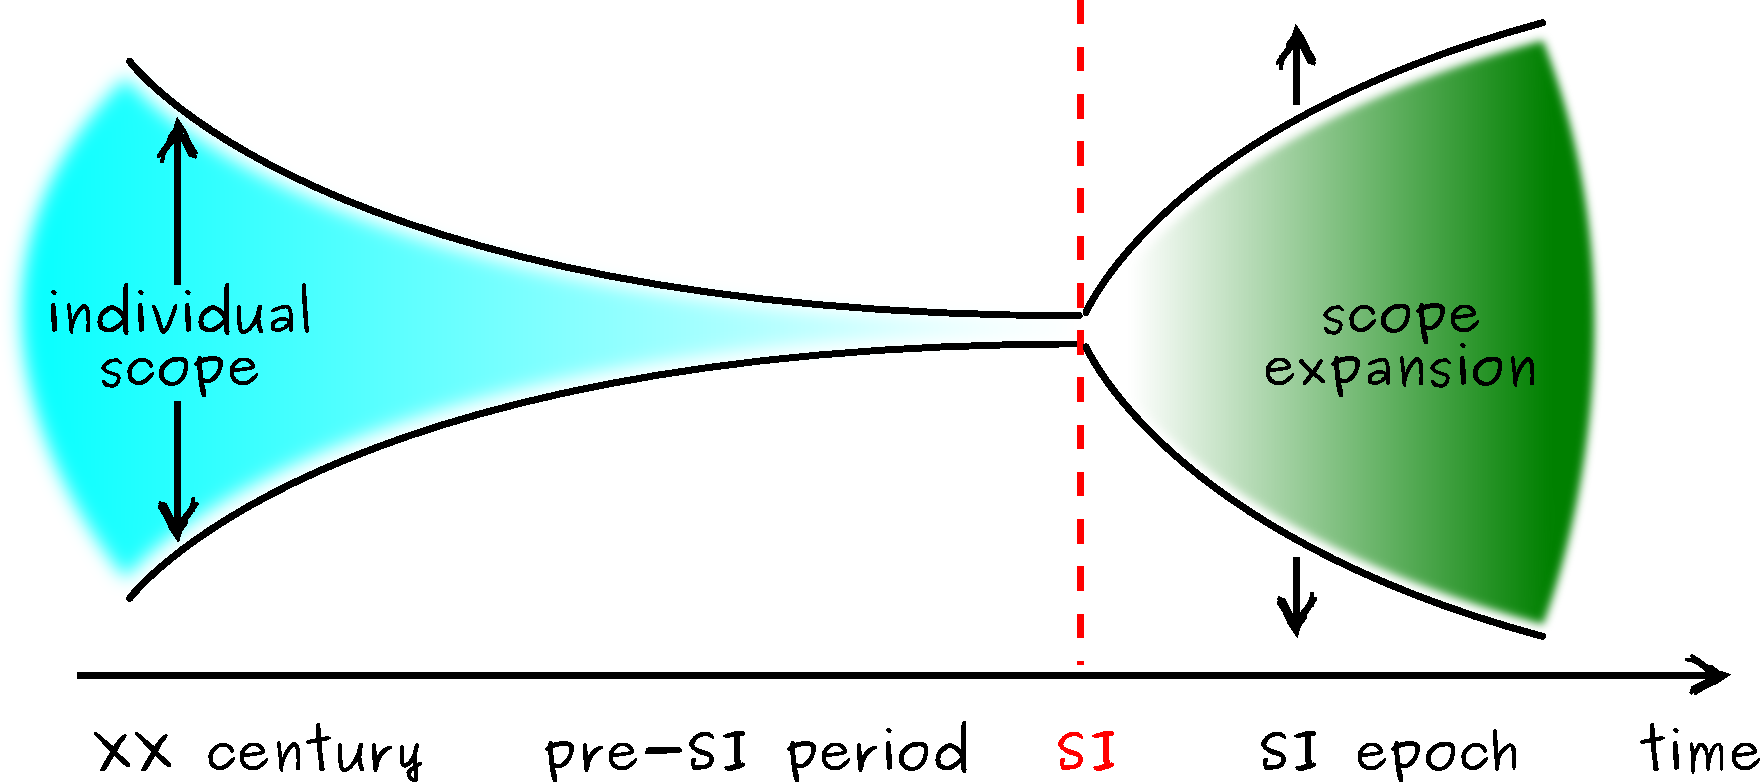
\includegraphics[width=1\textwidth]{scope}
    \caption{\label{fig:scope}Expansion of individual scientist's scientific scope in the SI epoch}
\end{figure}

\paragraph{Individual scale.}

At the individual scale, discovering new things make a lot of sense even though it is not on the forefront of SIS nor even of HS. So if in any case the utilitarian function of HS will vanish in the solved world, the excitement part will remain there if, of course, humans decide to keep the current mind settings.

\paragraph{SI as a senior colleague and mentor.}
SI can help us to move forward towards the frontiers of SIS by motivating, encouraging and guiding. With such a wise mentor and colleague we will be able to focus only on relevant questions and limit our distractions, i.e. it will not let us exploring dead ends. So, our personal progress, being directed, will be more efficient. However, the level of guidance can be adjusted, for example, instead of explicit guidance to the questions that matter, SI could give us hints that we could decipher: planets in a special arrangement, signs that we could notice during our morning rambling in a new city we are visiting, a quotation that we can occasionally read on a wall of a café where we drink our morning coffee. Of course, it all will be easier to implement in a digital universe.

When the questions of your scientific research are established and a path partially paved, SI can provide you with adapted reading, adjusted for your knowledge and brain's preferences in terms and in form, with probably some passages deliberately kept difficult, so it takes you some time to understand.
Or maybe you learn some new experimental techniques, tests them and finally deploy to understand some new (for you) in biology or particle physics.
So, you are encouraged to increase your mastering of the topic to pass some barriers and achieve the goal: prove a theorem, explore specific functions of some proteins or refine your understanding of strong interaction. Of course SI knows your current intellectual and work capacity, missing knowledge and your potential to make your own discovery and overcome the difficulty, so the problems can be perfectly adjusted and it can reveal to you that "you can do it". When we are sure that we can, then we truly can. It could be a finer message: "You can do it with 30\% probability." It would be more challenging but more rewarding. So, in such a set-up with a benevolent SI mentor, you can really surpass yourself and show the best of you. "I did believe that it was beyond your capacities, but you've finally proved this tricky theorem! Bravo!" - SI could deceive you with flattery in the end.

\paragraph{Science as a game/Playing in science.}
Humans have limited capacities in cognitive function, our speed is very limited as well as the number of tools we master and the broadness of topics we truly master. Even though we made tremendous progress in Science over the last couple of centuries, we won't be able to push the frontiers of science in the age of SI beyond the frontiers established by it. Nevertheless, we will be able ``to play'' in science. In any case it will be not about pushing science but if you wish it could be about believing\footnote{This could be done by adjustment of the brain or of its version uploaded into a simulation.} that you push it in an environment or entire universe crafted for you.

\paragraph{SI oracle and its priests and hypothesis of non-overlapping scientific questions\label{sec:oracle}}
Future scientist can serve as priests and priestess in a temple of SI oracle (analogous to a research center) by asking smart questions and documenting the answers into an ultimate book of knowledge (database). It could be a game in a solved world among other games of science we can imagine. Even though such activity of knowledge extraction could be seen as useful in the world of oracle only SI, it would loose most of its meaning in the world of agentic-like SI, because if we need a database of the integrality of scientific knowledge, in such a world, we will simply need to ask it to create such a database for us. Well at least for the list of questions about which the humankind can be curious during the upcoming millennium. Note here, that the list of questions which could be interesting for human individuals hypothetically is not necessarily a subset of the questions solved by SI to construct its world map and push its own SIS, i.e. $\text{HS} \not\subset \text{SIS}$. Those ``idle'' questions outside the SI's interest ($\text{HS} \setminus \text{SIS}$), could present an interesting playground for humans. However, the forced deployment of SI in these domains can of course expand the frontiers drastically, but would it worth it? Maybe, such rare islands of untouched by SI science would be the most valuable for human scientists. The SI can be forbidden in those lands.
Let's formulate properly this hypothesis.

% Usage
\begin{hypothesis}[Hypothesis of non-overlapping questions]\label{hyp:SI}
Questions of the Human-led Science does not fully overlap with the questions that Superintelligence explores to construct its world model. In other words, the questions of the Human-led Science minus questions explored by SI is not empty.
\end{hypothesis}



\begin{figure}[h!]
    \centering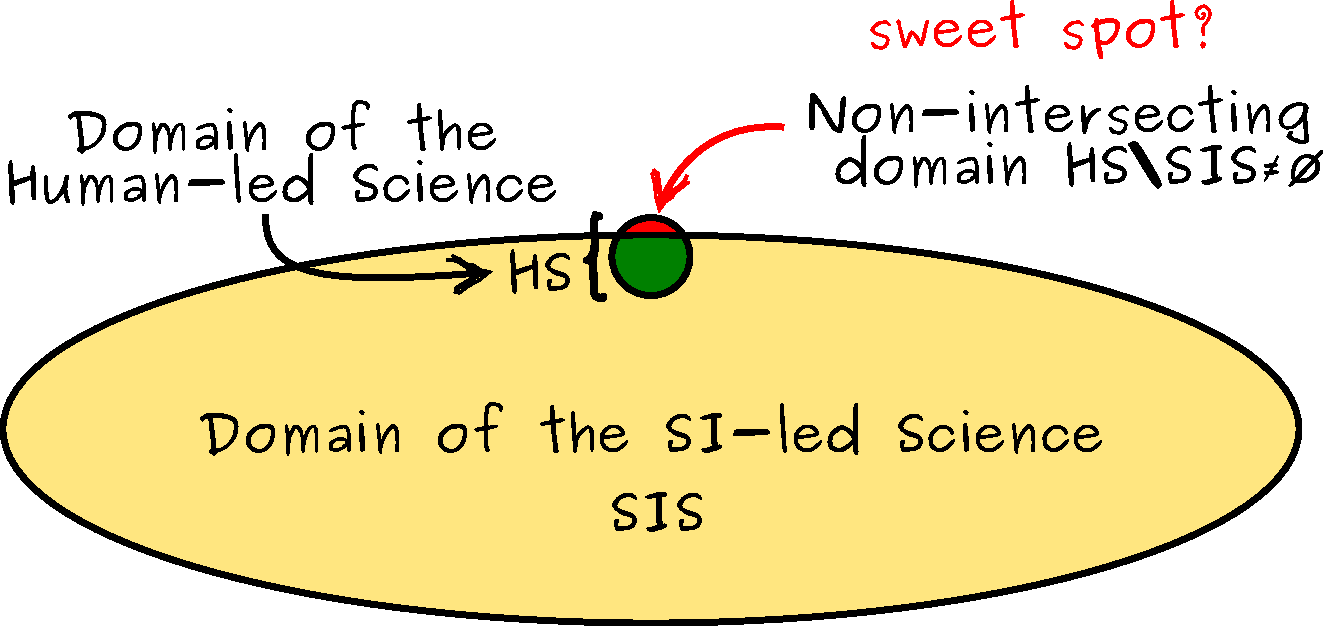
\includegraphics[width=0.7\textwidth]{intersections}
    \caption{\label{fig:intersection}Domains of Human-led Science (HS) and SI-led Science (SIS) and a sweet spot $\text{HS} \setminus \text{SIS} \ne \emptyset$ of ``idle'' scientific questions which do not interest SI for its world model but are interesting for individual humans. SI-led science could be forbidden within these spots to let the HS explore them.}
\end{figure}

But let's get back to the oracle/priest interaction. Even if there is strictly no utilitarian function of such kind of interaction with the oracle and ``manual'' filling the knowledge database, it could seem an interesting activity in a solved world and which would require a lot of intellectual efforts from humans. The priests and the priestess will not only asking questions but also trying to understand the answers and its implications. The task could be further (deliberately) complicated if the settings of the oracle are such that it does not try to simplify or even if it tends, as Oracle of Delph, to provide sometimes ambiguous and enigmatic answers which would for example require additional experiments and verifications. In other settings, for example, the oracle can answer only a limited number of questions per day or in total. Many aspiring rituals could be invented to accompany this worship in the temple of SI. Like in the ``Castalian Glass Bead Game'', being a priest or a priestess of the SI oracle could be an interesting intellectual activity in a solved world. And ultimately, such a database stored for eternity could be helpful in a scenario when SI lets us alone.

\paragraph{The Pace of SIS Progress}
Even with SI, scientific progress and discoveries will need some time. If ``Gedankenexperimente'' is not sufficient and some data collection is required, it can slow down the progress. Even for SIS, some experimental data are not easy to obtain and some technologies are not fast to implement. For example, construction of a new generation of LIGO for the study of gravitational waves  or of a (extra) Huge Hadron Collider to further push the frontiers of high-energy physics will require time. The same applies for new generations of fusion reactors. On the biological front, for example, studying some genetic information transmission in species other than drosophilas and mice may take decades. Therefore, it is clear that the progress of SIS in domains requiring data and experiments will be pinned, while in purely theoretical domains the progress can go very fast or even instantaneously from the human perspective. It will thus result in a non-smooth nature of the forefront knowledge. 

Nevertheless, even without access to the results of experiments, SI will be able to develop simultaneously alternative sciences based on different potential results experiments. As soon as the experiment in question provides conclusive results, alternative science branches will be eliminated, as in wave function collapse (see \Cref{fig:pinning})

On the social side, every (or almost) considerable update of the SIS's frontier can be publicly announced and be accompanied by a kind of press release. Top human experts can try to understand these milestones or take for granted some results.

\begin{figure}[ht!]
    \centering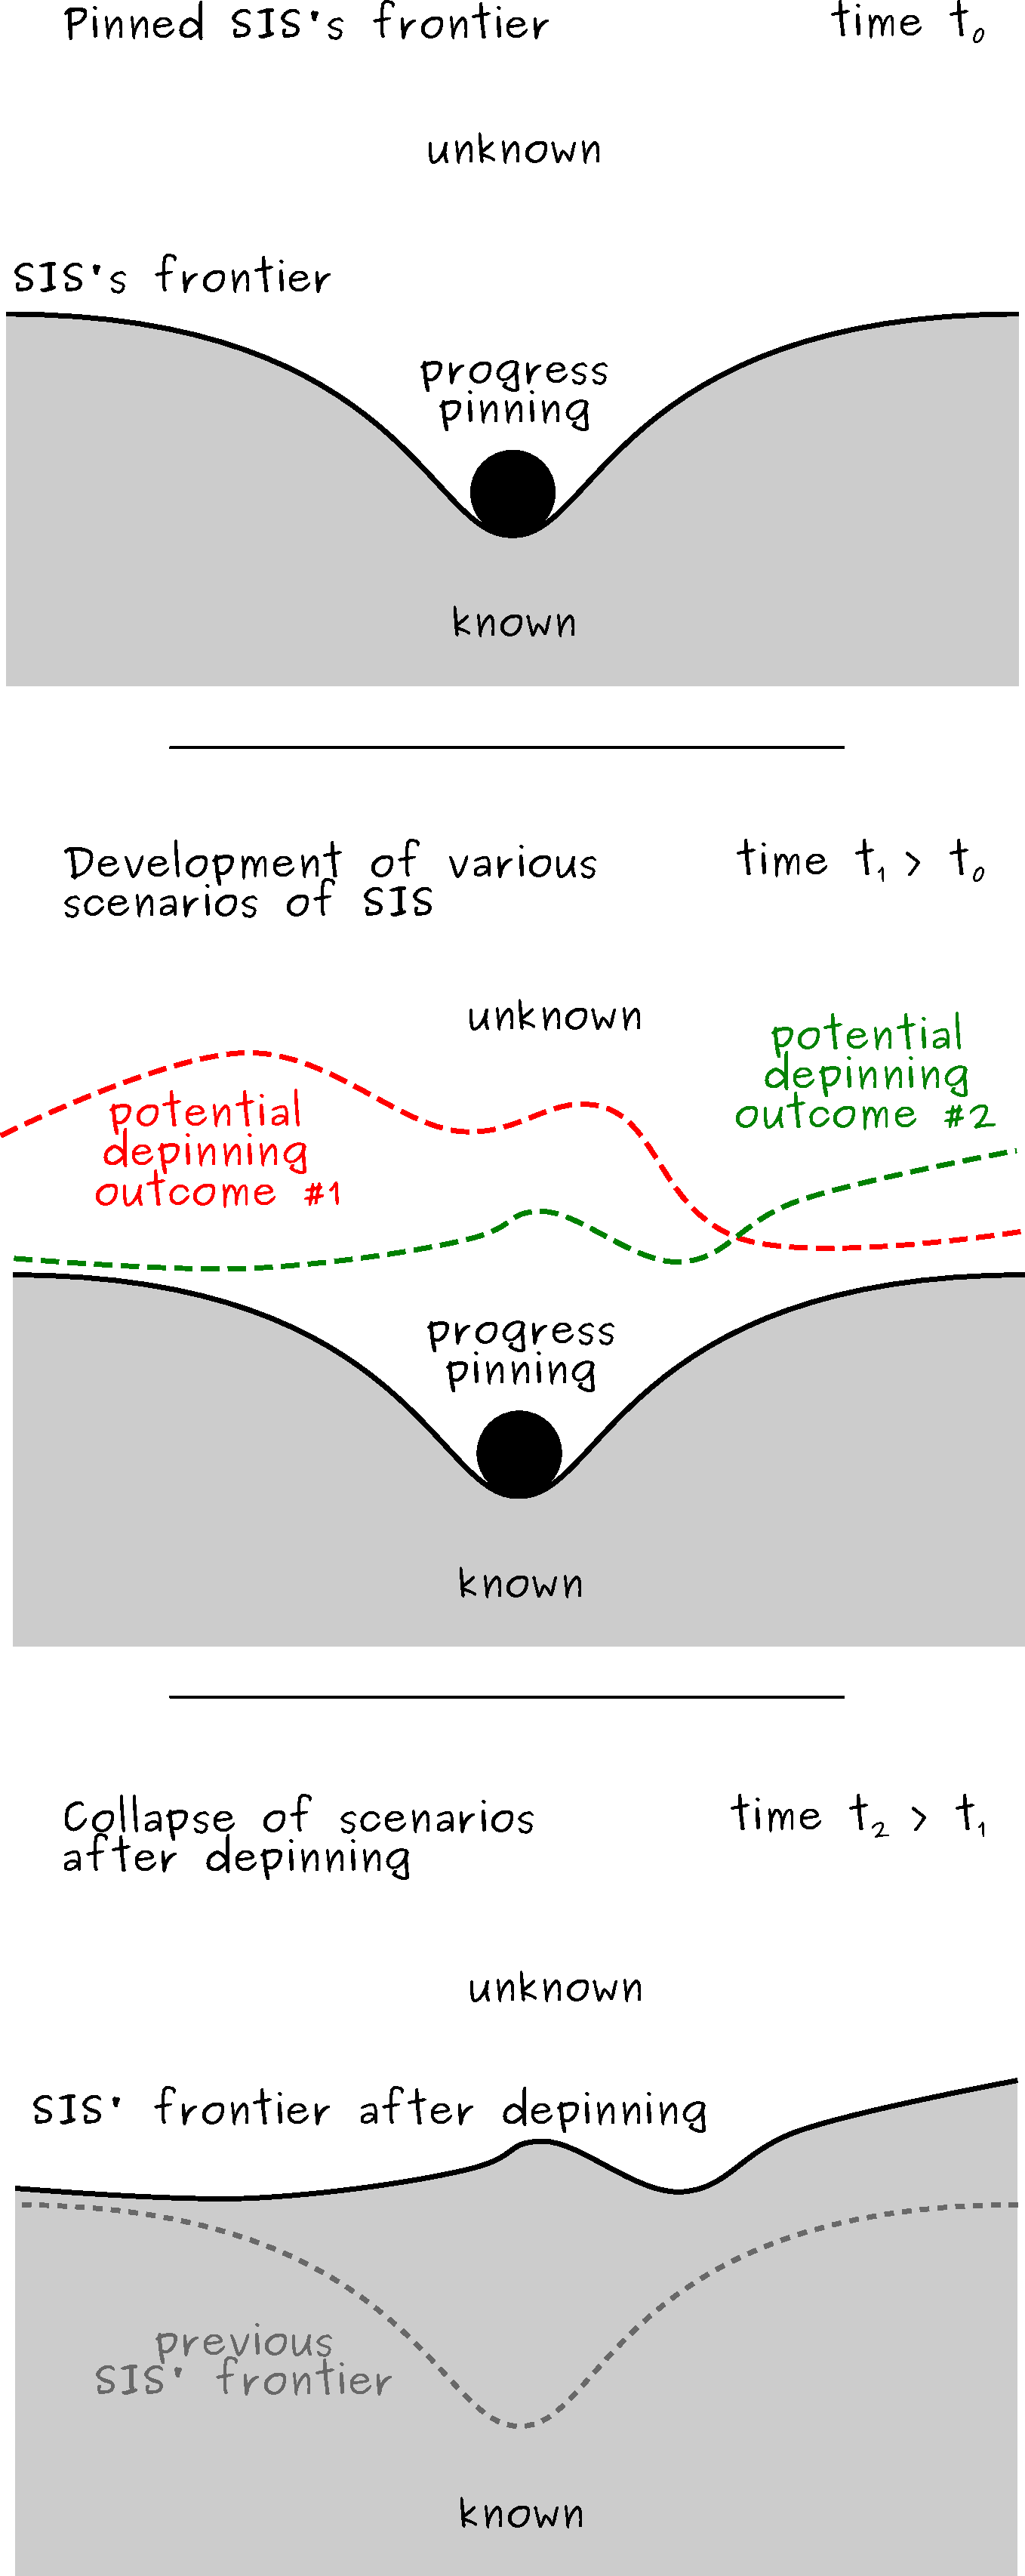
\includegraphics[width=0.6\textwidth]{depinning_2.pdf}
    \caption{\label{fig:pinning}Pinning and depinning event in SIS's frontier progress}
\end{figure}


\newpage

	\section{Introduction and main assumptions}

        \subsection{Oracle SI}

        \subsection{SI Capacity and Energy Efficiency}

        Notions: SI, HS - Human-led Science \nomenclature{HS}{Human-led Science} and Superintelligence Science (SIS) \nomenclature{SIS}{Superintelligence-led Science\footnote{Science constructed and advanced by the SI for the purpose of an accurate world model.}}, subgoals and World's most accurate model.

    \section{Scientific Landscape and its Frontiers}

        \subsection{Separation between HS and SIS}

        Sharing with humans, forbidden zones with high risks of black balls, World model and "праздные" scientific questions

        Domains left unexplored by SI, forced exploration

        \subsection{New Science}

        \subsection{Scientific Discoveries}

        Limits of SI's science: constant expansion or deliberately fixed limit or the full cover?

        \subsection{Cleaning up the science}

        \subsection{Race to the forefront}

        Advancement to the forefront (potentially moving one) and limits of human's brain capacities. Will be try to catch up with the most recent frontier or we will need to go through difficult paths to get there and appreciate/understand.

    \section{Humans in the Loop}

        \subsection{Game or not only?}

        Science as a game

        SI oracle and its priests

        \subsection{Enhancement/augmentation and Scope}

        Science-Optimized brains or minds

        SI as a senior wise colleague/mentor

        Scientific theaters

        Exploration of humans' brain

        Outer space exploration

        People will free to choose -- to be augmented and explore the forefronts of the science alongside with the SI or to be genuine people with maybe only light adjustments and make a slow pace progress towards the forefront and never reach it. But of course it is okay too.

        \subsection{Emulation of Scientific Progress}

        Individual universe

        \subsection{Meaning and Purpose}






\printbibliography

\end{document}
